\documentclass[12pt]{exam}
\usepackage{amsmath}
\usepackage{amssymb}
\usepackage{tikz}
\usepackage{wasysym}

\newcommand{\announce}[1]
{\vspace\baselineskip{\parindent0in {\bf #1}}}

\begin{document}
\pagestyle{empty}

%Top matter
{\parindent0in

\begin{center}
\huge \bf Final Exam
\end{center}

\makebox[0in][l]{Spring 2023}
\hfill
Abstract Algebra
\hfill
\makebox[0in][r]{Name: Rohan Jain}
}

\begin{questions}

\question Let $G$ be a ring in which $abc = cba$ for all $a, b, c \neq e$ in the group.  Show that $G$ is abelian.

\announce{Solution 1:} First we consider the case of $ab = e$. If this is true, then $a = b^{-1}$, so $ba = e = ab$. 

The second case is if $a,b \in G$ and $ab \neq e$, we have that $e = (ab)(ab)^{-1} = (ab)^{-1}(ba)$ by the problem statement. So $ab = ba$. 

By definition, we now have that $G$ is abelian. $\smiley$ 

\vspace{1cm}

\begin{minipage}[t]{5in}
\question Consider the group $\mathbf O$ of rigid motions of the octahedron.  There are 24 of them.  These consist of:
\begin{itemize}
\item The identity. (Total: 1)
\item Rotations of 90, 180, and 270 degrees about each axis through opposite vertices.  (Total: 9)
\item Rotations of 120 degrees clockwise or counterclockwise about an axis through the center of each pair of opposite faces.  (Total: 8)
\item Rotations of 180 degrees about an axis through opposite pairs of edges.  (Total: 12 edges, so 6 such pairs of axes)
\end{itemize}
\vspace{\itemsep}
\end{minipage}
\begin{minipage}[t]{1in} \vspace{0in}
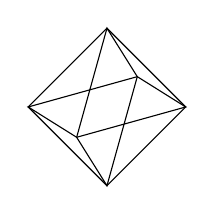
\begin{tikzpicture}
\draw (1,0,0) -- (0,1,0) -- (-1,0,0) -- (0,-1,0) -- cycle;
\draw (1,0,0) -- (0,0,1) -- (-1,0,0) -- (0,0,-1) -- cycle;
\draw (0,1,0) -- (0,0,1) -- (0,-1,0) -- (0,0,-1) -- cycle;
\end{tikzpicture}
\end{minipage}\\
There are clearly subgroups of orders 2, 3, and 4, since there are elements of each of those orders.  The next problem outlines a subgroup of order 8.  But what about the other possible orders?  The other proper divisors of 24 are 6 and 12.  Determine whether there are subgroups of order 6 or 12 on $\mathbf O$.  Either exhibit such a subgroup with that order or show that no such subgroup exists.  Do this for both order 6 and order 12!

\announce{Solution 2:} We start this problem by showing that the symmetries of a cube are isomorphic to the symmetries of an octahedron. This is because the cube and the octahedron form a dual pair. As such, they have the same symmetry groups. We can start by showing that the groups are congruent.

The basic idea is that the corners of the octahedron correspond to the faces of the cube and the faces of the octahedron correspond to the corners of the cube. If you look at each shape from a bird's eye view, you can label each triangular face of the octahedron in a similar fashion as to how you would label the corners of a cube. Then, corners of the octahedron could me labeled in a similar fashion to how you would label the faces of a cube. Performing the respective actions would allow you to track each corner and face the same way with both shapes. 
\\ \\ 
Here are the group of actions for the rigid motions of a cube:
\begin{itemize}
	\item The identity.
	\item Rotations of 90, 180, and 270 degrees about each axis through opposite faces.
	\item Rotations of 120 degrees clockwise or counterclockwise about an axis through the center of each pair of opposite corners.
	\item Rotations of 180 degrees about an axis through opposite pairs of edges. 
\end{itemize}
As you can count, this also has an order of 24. Additionally, this yields the following presentation for each of the groups.
$$\mathbf O = \langle a, b, c | a^4 = b^3 = c^2 = abc = e\rangle$$
$$S_4 = \langle a, b, c | a^4 = b^3 = c^2 = abc = e\rangle$$
In all of these, $a, b,$ and $c$ correspond to the 2nd, 3rd, and 4th bullet points listed for each of the groups. As such, we can conclude that $\mathbf O \cong S_4$. This yields the following answers to the question:

For order 6: The subgroup of order 6 of $S_4$ is $\boxed{S_3}$.

For order 12: The subgroup of order 12 of $S_4$ is $\boxed{A_4}$. 
\clearpage

\question There is a square on the ``equator'' of the octahedron.  This square can be rotated and flipped by the elements of $\mathbf O$.  So $\mathbf O$ has a subgroup isomorphic to $D_4$.  Determine whether this subgroup is normal.

\announce{Solution 3:} This subgroup is not normal. We have $(1 \; 2) \in S_4$ and $(1 \; 3) \in D_4$. However, $(1 \; 2)(1 \; 3)(1 \; 2) = (2 \; 3) \not\in D_4$. So, $D_4 \not \trianglelefteq S_4$. $\smiley$

\vspace{2cm}

\question The faces of the octahedron are painted in any of three different colors.  Two paintings are considered the same if one can be rotated into the other.  How many different paintings are there?

\announce{Solution 4:} Due to the previously shown isomorphism, this is the same as asking how many ways there are to color the corners of a cube. This was a previous homework problem that I am going to use Burnside's Lemma to solve. Here are permutations and respective counts. 



\begin{center}
	\begin{tabular}{ c | c | c }
		\textbf{Permutation} & \textbf{Count} & $|X_g|$ \\
		\hline
		Identity & 1 & $3^8$\\
		180 degree face rotation & 3 &$3^4$ \\
		90 degree rotation & 6 &$3^2$ \\
		180 degree edge rotation & 6 &$3^4$ \\
		120 degree edge rotation & 8 &$3^4$ \\
	\end{tabular}
\end{center}

Thus, the equation we get is $\frac{1}{24}(3^8 +3\cdot 3^4 + 6 \cdot 3^2 + 6\cdot 3^4 + 8\cdot 3^4) = \boxed{333}$. 

\vfill

\clearpage

\question A nonzero element $r$ of ring $R$ is called \emph{nilpotent} if $r^n = 0$ for some $n > 0$.  For example, 6 is nilpotent in $\mathbf Z_{32}$ because the powers of 6 are $6^2 = 36 \equiv 4$, $6^3 = 6\cdot4 = 24$, $6^4 = 6\cdot24 = 144 \equiv 16$, and $6^5 = 6\cdot16 = 96 \equiv 0$.

\begin{parts}
\part Prove that the set of all nilpotent elements in a commutative ring is an ideal.

\announce{Solution 5a:} There are three things we have to consider:
\begin{enumerate}
	\item Is 0 in the set?
	\begin{itemize}
		\item Yes, since $0^n = 0$ for all $n$.
	\end{itemize}
	\item If $a,b$ are in the set, is $a-b$ also nilpotent?
	\begin{itemize}
		\item Yes. If $a^x = 0$ and $b^y = 0$, then $(a-b)^{x+y} = 0$ by binomial expansion. Consider the value $a^jb^{x+y-j}$. If $j \geq x$, $a^j = 0$ so the whole term is 0. If $j < x$, then $b^{x+y-j} = 0$ and therefore the whole term is 0. So, by binomial theorem, it follows that $(a-b)^{x+y} = 0$ and that $a-b$ is nilpotent.
	\end{itemize}
	\item If $a$ is in the set and $r$ is in the ring, is $ra$ also nilpotent?
	\begin{itemize}
		\item Yes. If $a^n = 0$, then $(ra)^n = r^na^n = r^n0 = 0$ and the same goes for $ar$ because the ring is commutative.
	\end{itemize}
\end{enumerate}

Because the above criterion are satified, the set of nilpotent elements is an ideal. $\smiley$

\vspace{2cm}

\part Let $r \in R$ be nilpotent, with $R$ commutative, and let $J$ be a prime ideal.  Note that for some $n$, $r^n = 0 \in J$.  Use a little induction to prove that $r$ itself must be in $J$.

\announce{Solution 5b:} We will prove this by induction. Since $J$ is prime, for any element $ab \in J$, either $a \in J$ or $b \in J$. As such, if we have $\underbrace{rrr\cdots r}_{n \mbox{ times}} = r^n = 0 \in J$, we can say that either $r$ or $r^{n-1}$ is in $J$. If $r \in J$, then we're done. If $r^{n-1}$ is in $J$, we can split it into $r$ and $r^{n-2}$. We can continue this process until we get to $r$ itself, which must be in $J$ because $J$ is prime. $\smiley$

\end{parts}

\vfill

\fullwidth{The set of all nilpotent elements of a ring is called its \emph{nilradical} and by the second part of the problem, the nilradical is contained in the intersection of all prime ideas of a (commutative) ring.  The reverse inclusion is also true, but much harder to prove.  The case for noncommutative rings is much worse.}

\clearpage

\question
\begin{parts}
\part Let $D$ be a Euclidean domain with Euclidean valuation $v$.  Show that if $a$ and $b$ are associates, then $v(a) = v(b)$.

\announce{Solution 6a:} If $a$ and $b$ are associates, there exists a unit $u \in D$ such that $a=ub$. Since $v$ is a valuation, we have that $v(bu) \leq v(b) \Rightarrow v(a) \leq v(b)$. To continue, since $a=ub$, $b = u^{-1}a$ for some unit $u^{-1}$. Then we have that $v(au^{-1}) \leq v(a) \Rightarrow v(b) \leq v(a)$. Thus, $v(a) = v(b)$. $\smiley$

\vspace{2cm}

\part Now show that $v(ab) > v(a)$ if and only $b$ is not a unit.

\announce{Solution 6b:} If $b$ is a unit, then $ab$ and $a$ are associates so $v(ab) = v(a)$. But we assume $v(ab) > v(a)$ so $b$ cannot be a unit.

For the converse, suppose $b$ is not a unit. If $v(a) = v(ab)$, we use the Euclidean algorithm to get that $a = (ab)q + r$ where $r\neq0$ because $ab \nmid a$, in which case we can rewrite as $a(1 - bq) = r$. Since we are saying that $b$ is not a unit, $(1-bq) \neq 0$. And since $r \neq 0$, $v(a(1-bq)) = v(r) < v(a)$, which contradicts a condition for Euclidean norms. As such, we conclude that $v(ab) > v(a)$. $\smiley$
\end{parts}
\vfill

\end{questions}
\end{document}
